%%**************************************************************
%% Vorlage fuer Bachelorarbeiten (o.ä.) der DHBW
%%
%% Autor: Tobias Dreher, Yves Fischer
%% Datum: 06.07.2011
%%
%% Autor: Michael Gruben
%% Datum: 15.05.2013
%%**************************************************************
\documentclass[%
	enabledeprecatedfontcommands,
	pdftex,
	oneside,		% Einseitiger Druck.
	12pt,			% Schriftgroesse
	parskip=half,	% Halbe Zeile Abstand zwischen Absätzen.
	headsepline,	% Linie nach Kopfzeile.
	footsepline,	% Linie vor Fusszeile.
	abstracton,	    % Abstract Überschriften
	ngerman,		% Translator
]{scrreprt}
%!TEX root = ../dokumentation.tex

%
% Nahezu alle Einstellungen koennen hier getaetigt werden
%



%Seitengroesse
\usepackage{fullpage}

%Zeilenumbruch und mehr
\usepackage[activate]{microtype}

% Zeichencodierung
\usepackage[utf8]{inputenc}
\usepackage[T1]{fontenc}

% Zeilenabstand
\usepackage[onehalfspacing]{setspace}

% Index-Erstellung
\usepackage{makeidx}

% Lokalisierung (neue deutsche Rechtschreibung)
\usepackage[ngerman]{babel}

% Anführungszeichen 
\usepackage[babel,german=quotes]{csquotes}
%\usepackage[style=swiss]{csquotes}


% Spezielle Tabellenform fuer Deckblatt
\usepackage{longtable}
\setlength{\tabcolsep}{10pt} %Abstand zwischen Spalten
\renewcommand{\arraystretch}{1.5} %Zeilenabstand

% Grafiken
\usepackage{graphicx}

% Mathematische Textsaetze
%\usepackage{amsmath}
%\usepackage{amssymb}

% Pakete um Textteile drehen zu können, oder eine Seite Querformat anzeigen kann.
%\usepackage{rotating}
%\usepackage{lscape}

% Farben
\usepackage{color}
\definecolor{LinkColor}{rgb}{0,0,0.2}
\definecolor{ListingBackground}{rgb}{0.92,0.92,0.92}

\newcommand{\pdftitel}{AudiTim Dokumentation}
\newcommand{\autor}{Vorname Nachname}
\newcommand{\arbeit}{Bachelorarbeit}

% Titel, Autor und Datum
\title{\titel}
\author{\autor}
\date{\datum}

% PDF Einstellungen
\usepackage[%
	pdftitle={\pdftitel},
	pdfauthor={\autor},
	pdfsubject={\arbeit},
	pdfcreator={pdflatex, LaTeX with KOMA-Script},
	pdfpagemode=UseOutlines, % Beim Oeffnen Inhaltsverzeichnis anzeigen
	pdfdisplaydoctitle=true, % Dokumenttitel statt Dateiname anzeigen.
	pdflang=de % Sprache des Dokuments.
]{hyperref} 

% (Farb-)einstellungen für die Links im PDF
\hypersetup{%
	colorlinks=true, % Aktivieren von farbigen Links im Dokument
	linkcolor=LinkColor, % Farbe festlegen
	citecolor=LinkColor,
	filecolor=LinkColor,
	menucolor=LinkColor,
	urlcolor=LinkColor,
	bookmarksnumbered=true % Überschriftsnummerierung im PDF Inhalt anzeigen.
}

% Literaturverweise nach Harvard (mit deutschem und)
\usepackage[dcucite]{harvard}
\renewcommand{\harvardand}{und}

% Verschiedene Schriftarten
%\usepackage{goudysans}
%\usepackage{lmodern}
%\usepackage{libertine}
\usepackage{palatino} 

% Hurenkinder und Schusterjungen verhindern
% http://projekte.dante.de/DanteFAQ/Silbentrennung
\clubpenalty=10000
\widowpenalty=10000
\displaywidowpenalty=10000

% Quellcode
\usepackage{listings}
\lstloadlanguages{Java}
\lstset{%
	language=PHP,		 	 % Sprache des Quellcodes
	%numbers=left,           % Zelennummern links
	stepnumber=1,            % Jede Zeile nummerieren.
	numbersep=5pt,           % 5pt Abstand zum Quellcode
	numberstyle=\tiny,       % Zeichengrösse 'tiny' für die Nummern.
	breaklines=true,         % Zeilen umbrechen wenn notwendig.
	breakautoindent=true,    % Nach dem Zeilenumbruch Zeile einrücken.
	postbreak=\space,        % Bei Leerzeichen umbrechen.
	tabsize=2,               % Tabulatorgrösse 2
	basicstyle=\ttfamily\footnotesize, % Nichtproportionale Schrift, klein für den Quellcode
	showspaces=false,        % Leerzeichen nicht anzeigen.
	showstringspaces=false,  % Leerzeichen auch in Strings ('') nicht anzeigen.
	extendedchars=true,      % Alle Zeichen vom Latin1 Zeichensatz anzeigen.
	captionpos=b,            % sets the caption-position to bottom
	backgroundcolor=\color{ListingBackground} % Hintergrundfarbe des Quellcodes setzen.
}
\usepackage{xcolor}

% Define JavaScript language for listings
\lstdefinelanguage{JavaScript}{
  keywords={break, case, catch, continue, debugger, default, delete, do, else, finally, for, function, if, in, instanceof, new, return, switch, this, throw, try, typeof, var, void, while, with, let, const, yield, import, export, class, extends, super},
  keywordstyle=\color{blue}\bfseries,
  ndkeywords={boolean, throw, implements, import, this},
  ndkeywordstyle=\color{darkgray}\bfseries,
  identifierstyle=\color{black},
  sensitive=false,
  comment=[l]{//},
  morecomment=[s]{/*}{*/},
  commentstyle=\color{gray}\ttfamily,
  stringstyle=\color{red}\ttfamily,
  morestring=[b]',
  morestring=[b]"
}

% General listings style
\lstset{
  language=JavaScript,
  backgroundcolor=\color{gray!10},
  basicstyle=\ttfamily\small,
  numbers=left,
  numberstyle=\tiny\color{gray},
  stepnumber=1,
  numbersep=8pt,
  showstringspaces=false,
  breaklines=true,
  frame=single,
  tabsize=2
}

% Glossar
\usepackage[
	nonumberlist, %keine Seitenzahlen anzeigen
	%acronym,      %ein Abkürzungsverzeichnis erstellen
	%section,     %im Inhaltsverzeichnis auf section-Ebene erscheinen
	toc,          %Einträge im Inhaltsverzeichnis
]{glossaries}

%Akronyme
\usepackage[printonlyused,footnote]{acronym}
\usepackage{adjustbox} % in die Präambel

% Fussnoten
\usepackage[perpage, hang, multiple, stable]{footmisc}

%Bildpfad
\graphicspath{{images/}}

%nur ein latex-Durchlauf für die Aktualisierung von Verzeichnissen nötig
\usepackage{bookmark}

%Gleitumgebungen (Bilder, Tabellen, usw\ldots) lassen sich mit H an genau der
% definierten Stelle platzieren
\usepackage{float}

% für die vertikale Platzierung von Text in Tabellen
\usepackage{array}

% für die Darstellung des Euro-Symbols
\usepackage[right]{eurosym}

% für textumflossene Grafiken
\usepackage{wrapfig}

% eine Kommentarumgebung "k" (Handhabe mit \begin{k}<Kommentartext>\end{k},
% Kommentare werden rot gedruckt). Wird \% vor excludecomment{k} entfernt,
% werden keine Kommentare mehr gedruckt.
\usepackage{comment}
\specialcomment{k}{\begingroup\color{red}}{\endgroup}
%\excludecomment{k}

\usepackage{longtable}
\usepackage{adjustbox}
\usepackage{caption} % optional, für schönere Tabellenbeschriftung
\usepackage{pdflscape} % in der Präambel

% Ab jetzt können auch Umlaute verwendet werden

%falls pdftitel = titel der Arbeit
\newcommand{\titel}{\pdftitel}
%bei unterschiedlichen Titeln
%\newcommand{\titel}{AudiTim Dokumentation}
\newcommand{\martrikelnr}{5}
\newcommand{\kurs}{INF2023AI}
\newcommand{\datumAbgabe}{September 2025}
\newcommand{\firma}{Aaron Reiber, Jan-David Oberländer,}
%\newcommand{\firmenort}{Firmenort}
%\newcommand{\abgabeort}{Abgabeort}
%\newcommand{\abschluss}{Bachelor of Engineering}
%\newcommand{\studiengang}{Studienganges Vorderasiatische Archäologie}
\newcommand{\dhbw}{Heidenheim}
\newcommand{\betreuer}{Luca Müller, Moritz Flaig}
%\newcommand{\gutachter}{Dr. Silvana Koch-Mehrin}
\newcommand{\zeitraum}{10 Wochen}
\newcommand{\arbeitsart}{\arbeit}

\makeglossaries
\input{ads/glossary}

\begin{document}

	% Deckblatt
	\begin{spacing}{1}
		%!TEX root = ../dokumentation.tex

\begin{titlepage}
	\begin{longtable}{p{.4\textwidth} p{.4\textwidth}}
	  {
\includegraphics[height=2.6cm]{images/logo.png}} & 
	  {\includegraphics[height=2.6cm]{images/dhbw.png}}
	\end{longtable}
	\enlargethispage{20mm}
	\begin{center}
	\vspace*{12mm}	{\LARGE\bf \titel }\\
    \vspace*{12mm} SE-Projekt\\
    \vspace*{3mm} des Studiengangs\\
    \vspace*{3mm} Allgemeine Informatik\\
    \vspace*{12mm} an der Dualen Hochschule Baden-Württemberg, Campus Heidenheim\\
	  %\vspace*{12mm}	{\large\bf \arbeit}\\
	  %\vspace*{12mm}	für die Prüfung zum\\
	  %\vspace*{3mm} 	{\bf \abschluss}\\
	  %\vspace*{12mm}	des \studiengang\\
	  %\vspace*{3mm} 	an der Dualen Hochschule Baden-Württemberg \dhbw\\
	  %\vspace*{12mm}	von\\
	  %\vspace*{3mm} 	{\large\bf \autor}\\
	  %\vspace*{12mm}	\datumAbgabe\\
	  \begin{center}
  \textit{Diese Dokumentation entstand im Rahmen des Software-Engineering-Projekts 
  an der Dualen Hochschule Baden-Württemberg. 
  Sie beschreibt die Konzeption und Umsetzung von AudiTim, einem verteilten System zur akustischen Raumüberwachung, 
  dessen Ziel die Erfassung, Speicherung und Visualisierung von Lautstärkedaten in einem Vorlesungsraum ist.}
\end{center}
	\end{center}
	\vfill
	\begin{spacing}{1.2}
	\begin{tabbing}
		mmmmmmmmmmmmmmmmmmmmmmmmmm     \= \kill
		\textbf{Bearbeitungszeitraum}  \>  \zeitraum\\
		\textbf{Gruppe, Kurs}  \>  \martrikelnr, \kurs\\
		\textbf{Gruppenmitglieder}      \>  \firma\\
		\textbf{}              \>  \betreuer\\
		%\textbf{Gutachter}             \>  \gutachter
	\end{tabbing}
	\end{spacing}
\end{titlepage}

	\end{spacing}
	\newpage

	\renewcommand{\thepage}{\Roman{page}}
	\setcounter{page}{1}

	% Sperrvermerk
	%\input{ads/sperrvermerk}
	%\newpage
	
	% Erklärung
	%\input{ads/erklaerung}
	%\newpage

	% Abstract
	%\input{ads/abstract}
	%\newpage

	\pagestyle{plain}

	% Inhaltsverzeichnis
	\begin{spacing}{1.1}
		\setcounter{tocdepth}{1}
		%für die Anzeige von Unterkapiteln im Inhaltsverzeichnis
		%\setcounter{tocdepth}{2}
		\tableofcontents
	\end{spacing}
	\newpage

	\renewcommand{\thepage}{\arabic{page}}
	\setcounter{page}{1}
	
	% Inhalt
	\chapter{Einleitung}

Im Rahmen des Software-Engineering-Projekts wird in einem Team ein System zur akustischen Raumüberwachung entwickelt. 
Ziel des Projekts ist die kontinuierliche Erfassung und spätere Analyse der Lautstärkeverteilung in einem typischen Vorlesungsraum über den Zeitraum mehrerer Tage hinweg.

\section{Projektüberblick}

Die Umsetzung erfolgt nach agilen Prinzipien unter Anwendung von Scrum, wobei die jeweiligen Sprints von Freitag bis Freitag festgelegt wurden. 

Die technische Architektur sieht den Einsatz von vier Mikrocontroller-Einheiten (ESP32) vor, die jeweils mit einem Mikrofon oder einem Dezibel-Messsensor ausgestattet werden. 
Die Geräte werden in den vier Ecken des Vorlesungsraums positioniert, um eine möglichst flächendeckende Abdeckung des Raumes zu gewährleisten. Über ein Kommunikationsprotokoll tauschen sich die ESPs untereinander aus und 
senden die gesammelten Messdaten gemeinsam an ein zentrales Backend.

\section{Ziele und Motivation}

Ziel ist es, ein skalierbares und robustes System zu entwickeln, das Lautstärkepegel über einen längeren Zeitraum erfassen kann. Die gesammelten Daten sollen im Backend gespeichert und im Nachgang analysiert werden. 
Hierbei sind verschiedene Darstellungsformen wie etwa Heatmaps oder zeitbasierte Diagramme denkbar, um Muster oder Auffälligkeiten im akustischen Verhalten des Raumes sichtbar zu machen.

\section{MVP und Qualitätsmerkmale}

Im Rahmen des MVPs soll ein verteiltes System zur akustischen Raumüberwachung auf Basis von vier Mikrocontrollern der ESP-Serie entwickelt werden. 
Jeder ESP wird über ein extern angeschlossenes Mikrofon verfügen, mit dem kontinuierlich Lautstärkedaten erfasst werden. Drei der Module sollen ihre Messwerte mithilfe des ESP-NOW-Protokolls an eine zentrale Einheit übermitteln, 
die zusätzlich eigene Daten erfasst. Die aggregierten Informationen aller vier Einheiten werden in festen Intervallen über das MQTT-Protokoll an einen Server gesendet und dort zeitsynchron in einer InfluxDB gespeichert. 
Über eine REST-API sollen die Daten einem Angular-basierten Web-Frontend zur Visualisierung der akustischen Messwerte zur Verfügung gestellt werden.

\begin{center}
  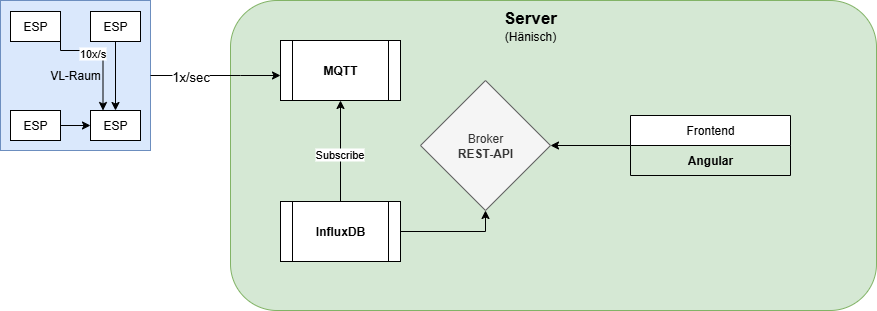
\includegraphics[width=1\textwidth]{../images/MVP/MVPVisualisierung.png}
\end{center}

Aufgrundlage des MVPs sollen die folgenden Qualitätsmerkmale sichergestellt werden:
\begin{itemize}
    \item \textbf{Echtheit \& Qualität der Daten:}
    Nur qualitativ "gute" Daten z.B. durch optimierte Mikrofongehäuse ermöglichen realistische Messwerte und damit eine sinnvolle Analyse der akustischen Verhältnisse im Raum.
    \item \textbf{Accountability der Daten:}
    Es muss nachvollziehbar sein, welche Sensoren zu welchem Zeitpunkt welche Daten erfasst haben.
\end{itemize}

	\input{content/02kapitel}
	\chapter{Auswahl und Bewertung der Hard- und Softwarekomponenten}

\section{Hardwarekomponenten}

\subsection{Mikrofonmodule}

Zur Erfassung des Lautstärkepegels wurden drei unterschiedliche Mikrofonmodule in Betracht gezogen. 
Der erste Sensor ist ein kostengünstiges Modul "GY-MAX4466" (ca.\ 4\,€), das ursprünglich als Klatschsensor konzipiert wurde. 
Der zweite Sensor ist das \textit{Sound Level Meter V2.0} von DFRobot (ca.\ 40\,€), das über zusätzliche Hardware zur Signalverarbeitung verfügt und den Schalldruckpegel bereits gefiltert und bereinigt im dBA-Format ausgibt.
Der dritte in Betracht gezogene Sensor ist ein handelsübliches DB-Messgerät (ca.\ 20\,€), das jedoch nicht für die Integration in das Projekt geeignet ist, da es keine digitale Schnittstelle bietet und somit nicht direkt mit dem ESP32 kommunizieren kann.
Dieser Sensor wird daher zur Überprüfung der Ergebnisse verwendet, ist aber nicht für die direkte Integration in das Projekt vorgesehen.

Da die absolute Einheit (dBA) für die Auswertung im Rahmen eines 3D-Diagramms nicht zwingend erforderlich ist, wurde der Fokus auf die Vergleichbarkeit der analogen Ausgangssignale gelegt. 
Beide Sensoren wurden gleichzeitig an einem ESP32 betrieben und ihre Ausgangssignale mithilfe des \textit{Serial Plotter} in Echtzeit visualisiert. 
Dabei zeigte sich, dass die Kurvenverläufe bei normalen Sprachgeräuschen nahezu identisch sind. 
Lediglich bei impulsartigen Geräuschen mit sehr geringer Distanz (z.\,B.\ Klatschen oder Klopfen) erzeugt das günstigere Mikrofon deutlich stärkere Peaks, während diese durch den DFRobot-Sensor wirksam herausgefiltert werden.

\begin{center}
  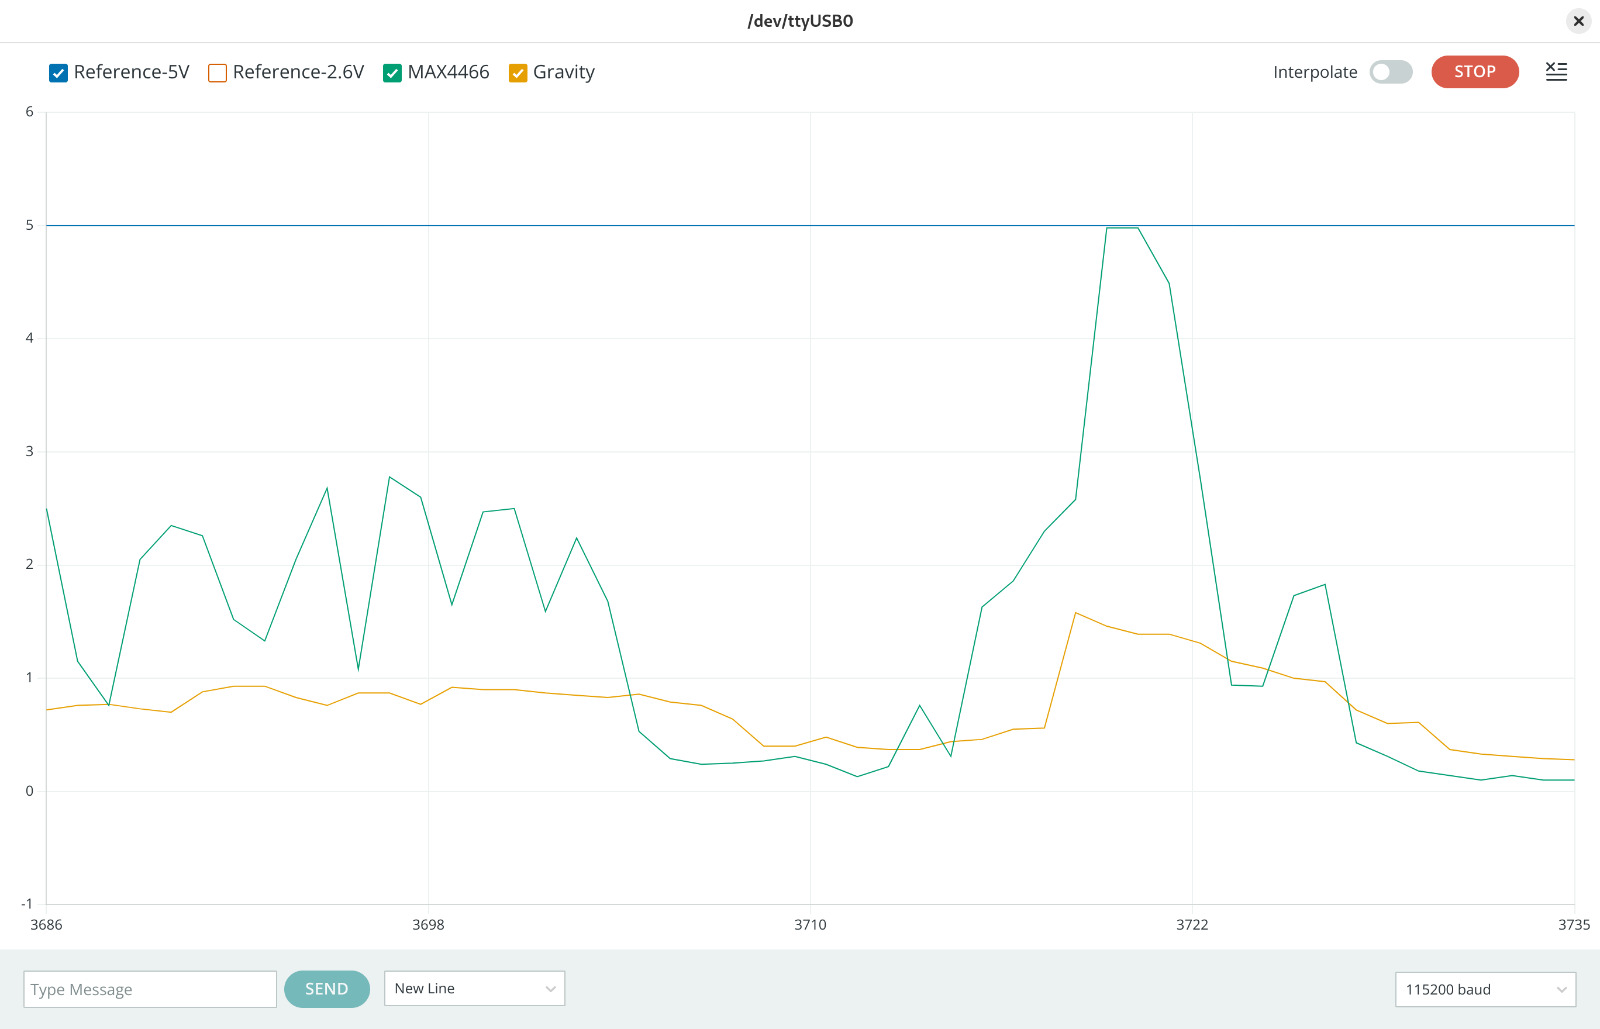
\includegraphics[width=1\textwidth]{../images/Sensorvergleich/PeekSensorVergleich.jpeg}
\end{center}
\begin{center}
  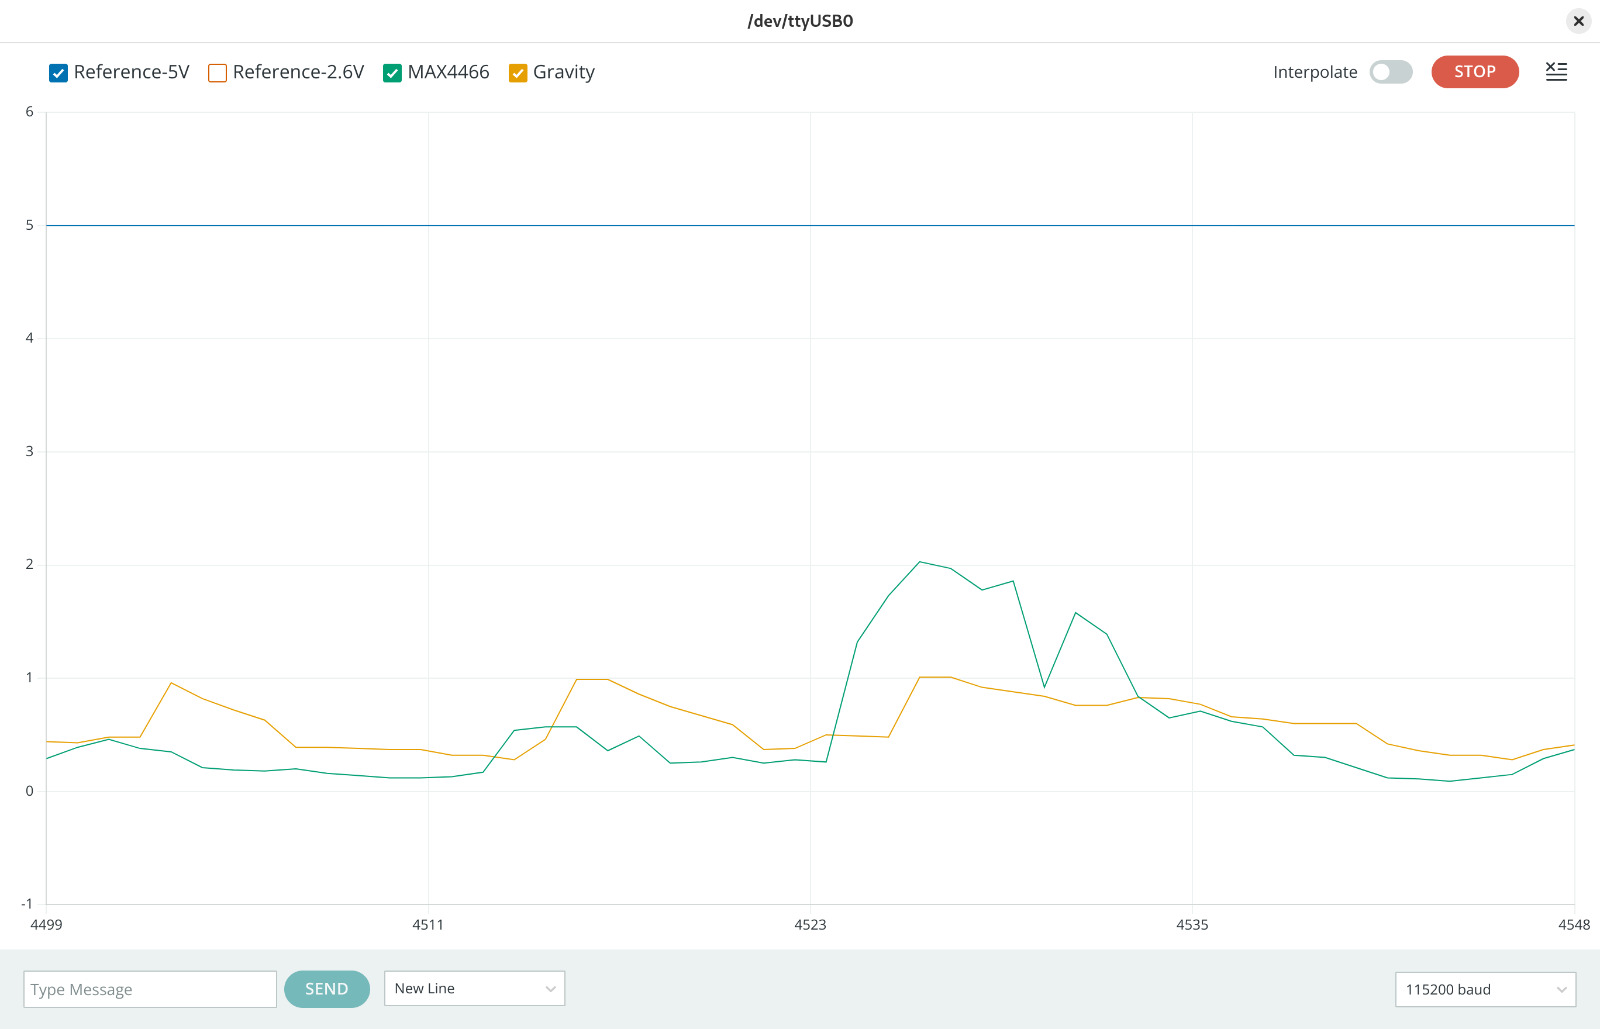
\includegraphics[width=1\textwidth]{../images/Sensorvergleich/StaticSensorVergleich.jpeg}
\end{center}

Hier sind die Sensorwerte des günstigeren Klatschsensors (grün), sowie die des Teureren Dba sensors (gelb) dargestellt. Die In Blau dargestellte 5v Referenzlinie stellt den Maximalwert da, welcher von den Sensoren zurückgegeben werden kann.

Da die in den Vergleichsdiagrammen dargestellten Abweichungen bei größerem Abstand deutlich abnehmen und im Anwendungsfall als vernachlässigbar eingestuft werden können, wurde entschieden, den günstigeren Sensor zu verwenden. 
Um mögliche Reststörungen dennoch weiter zu reduzieren, ist geplant, eine mechanische Dämpfung oder Abschirmung am Sensor zu testen.

Insgesamt konnte festgestellt werden, dass der günstigere Sensor trotz fehlender dBA-Ausgabe für die angestrebte Visualisierung ausreichend präzise Ergebnisse liefert und somit für den weiteren Projektverlauf verwendet wird.

\section{Softwarekomponenten}
\subsection{Entwicklungsumgebungen}

Zu Beginn des Projekts wurden zwei gängige Entwicklungsumgebungen für die Programmierung von Mikrocontrollern evaluiert: die klassische \textit{Arduino IDE}, welche auch von den betreuenden Dozierenden empfohlen wurde, sowie die moderne, zunehmend verbreitete \textit{PlatformIO}-Erweiterung für Visual Studio Code.

Im Projektteam wird plattformübergreifend mit Linux, Windows 10 und Windows 11 gearbeitet. Beide Entwicklungsumgebungen sind grundsätzlich mit allen eingesetzten Betriebssystemen kompatibel. Zur Prüfung der technischen Umsetzbarkeit wurden zwei separate Repositories eingerichtet, in denen jeweils einfache Testprojekte zur Ansteuerung eines ESP32 implementiert wurden.

Beide IDEs konnten den Mikrocontroller erfolgreich ansprechen. PlatformIO bietet durch seine deklarative Verwaltung von Bibliotheken und Abhängigkeiten Vorteile in Bezug auf Reproduzierbarkeit und Build-Konsistenz. In der Praxis kam es jedoch auf einem System im Team zu anhaltenden technischen Problemen mit PlatformIO, die nicht zufriedenstellend gelöst werden konnten.

Um eine einheitliche und zuverlässige Entwicklungsgrundlage für alle Teammitglieder sicherzustellen, fiel die Entscheidung letztlich zugunsten der \textit{Arduino IDE}. Diese ermöglicht eine barrierefreie Mitarbeit aller Beteiligten, auch wenn sie im Funktionsumfang nicht ganz an PlatformIO heranreicht.

\subsection{Kommunikationsmethode}
ESP-NOW wurde ausgewählt, da es im Vergleich zu anderen Protokollen einen deutlich geringeren Overhead besitzt und dadurch eine schnellere und effizientere Datenübertragung ermöglicht. Die Struktur ist weniger komplex, was die Implementierung vereinfacht und die Fehleranfälligkeit reduziert. 
Dadurch wird das System insgesamt robuster und zuverlässiger:
ESP-Now ist ein Kommunikationsprotokoll von Espressif, das speziell für die ESP32- und ESP8266-Chips entwickelt wurde. Es verwendet die 2,4 Ghz Frequenz, welche eigentlich für WiFi Kommunikation verwendet wird. 
Im Gegensatz zu anderen Protokollen sind die Nachrichten auf Schicht 2 des ISO-OSI-Modells. Keine IP-Adressen sondern nur MAC-Adressen. Die ESPs müssen sich dafür im gleichen Kanal befinden. Die 2,4 Ghz Frequenz hat grundsätzlich nur 3 Nutzbare Kanäle. 
Der zu verwendene Kanal muss von dem "AI401" Wlan Netz übernommen werden.Es ist mit relativ wenig Code möglich eine große Menge an Daten in sehr Kurzen Zeitabschnitten zu senden. Theoretisch ist eine Datenübertragung von 1 bis 2 Mbps möglich. 
Die Nachrichtenlänge ist auf 250 Byte pro Paket beschränkt. Da unsere Nachrichten nur wenige Bit lang sind, haben wir hier keine Probleme. 
Das Protokoll hat keine festgelegten Sender/Empfänger Rollen. Jeder ESP kann senden und empfangen. In unserem Beispiel senden aber 3 ESPs und ein Edge-Device empfängt alle Daten. 
Es wird 10 mal pro Sekunde der Lautstärkepegel erfasst und gesendet.

\subsection{ESP32}
Die ESP-Module bieten im Vergleich zu klassischen Arduinos eine integrierte WLAN-Funktionalität und unterstützen direkt das ESP-NOW-Protokoll. Dadurch entfällt zusätzlicher Hardware- oder Softwareaufwand für die Netzwerkkommunikation.
In Kombination mit ESP-NOW ergibt sich somit eine kompakte, performante und zuverlässige Lösung.

\subsection{Frontend}
Für die Umsetzung des Frontends wurde das Framework \textit{Angular} gewählt. 
Diese netschiedung basiert auf technischen Faktoren und persönlichen Preferenzen. 
Angular bietet eine klare Struktur durch komponentenbasiertes Design und ist für die moderne Webentwicklung gut geeignet.
Es erleichtert die Wiederverwendbarkeit von eigenen aber auch externen UI-Elementen und unterstützt eine saubere Trennung von Logik und Darstellung. 

Im Vergleich dazu ist \textit{React} ein von Meta entwickeltes UI-Framework. 
\textit{Angular} und \textit{React} haben beide eine komponentenbasierte Architektur. 
Diese Komponenten sind innerhalb anderer Komponenten wiederverwendbar und somit endlos wiederverwertbar. 
Beide sind Open Source. Daher haben React und Angular große Entwicklergemeinschaften, die die Ressourcen regelmäßig erweitern.
Angular ist ein vollwertiges Framework, während React eine JavaScript-Bibliothek ist. 
Deshalb muss React mit einem Framework gepaart werden, um eine schnelle, schöne und kompatible Benutzeroberfläche zu erstellen. 
\cite{kinsta2023angularvreact}

Da außerdem im Team bereits umfangreiche Erfahrung mit diesem Framework vorhanden war, fiel die Entscheidung zugunsten von Angular.
Das Frontend läuft in einem eigenen Docker-Container und kommuniziert, über ein internes Netzwerk, mit dem separat laufenden Backend-Container. 
So bleibt die Architektur modular, skalierbar und einfach wartbar.

Die Darstellung der Daten wird über Angular-Komponenten realisiert,
die Visualisierung in einfachen Liniendiagrammen wird mit der ng2-charts-Bibliothek ermöglicht.
\begin{center}
  \includegraphics[width=1\textwidth]{../images/LinechartFE.png}
\end{center}

\subsection{Backend}
Das Backend wurde mit Node.js und dem minimalistischen Framework Express.js umgesetzt. 
Express ist das am weitesten verbreitete Node.js-Framework für Webserver und APIs. 
Es bietet eine ausgereifte Middleware-Architektur, die sehr flexibel und modular ist. 
Im Vergleich zu ähnlich minimalistischen Frameworks wie Koa, 
das von den gleichen Entwicklern stammt, 
bietet Express mehr out-of-the-box Funktionalitäten und eine größere Community mit umfangreichen Plugins und Support. \cite{betterstack2025koavsexpress,appventurez2025nodejsframework}

Koa hingegen ist moderner und basiert stärker auf ES6 Features wie async/await, was den Code oft sauberer macht. 
Allerdings ist Koa weniger „batteries included“ und erfordert mehr Initialaufwand und zusätzliche Libraries, 
um Funktionen bereitzustellen, die Express standardmäßig mitbringt. 
Für dieses Projekt, welches einen schnellen Einstieg, umfangreiche Dokumentation und stabile Middleware braucht, 
ist Express daher die pragmatischere Wahl.
Zudem sind Gruppenmitglieder bereits mit Express vertraut, was die Einarbeitungszeit verkürzt und die Produktivität steigert. 

Die Anbindung an eine InfluxDB erfolgt über die offizielle Client-Bibliothek. 
Neben dem Abrufen historischer Sensorwerte werden auch Funktionen zum Schreiben von Dummy-Daten bereitgestellt.
Diese werden, solange die Verbindung zu den wirklichen Sensorwerten noch nicht hergestellt ist, zum Testen verwendet.

Für die Speicherung der Sensordaten wurde InfluxDB gewählt. 
Eine Zeitreihen-Datenbank, die speziell für viele konsekutive Datenströme optimiert ist. 
InfluxDB bietet eine simple API und gutes visuelles UI, ohne dass viel Konfiguration nötig ist.
Im Vergleich zu einer relationalen Datenbank wie TimescaleDB, die auf PostgreSQL basiert,
ist InfluxDB deutlich einfacher zu handhaben und benötigt weniger Overhead für die Konfiguration.
Um eine TimescaleDB sicher zum laufen zu bringen, sind komplexe Zugriff-Skripte benötigt, um die Benutzer zu verwalten.
InfluxDB hingegen arbeitet mit einem einfachen Benutzer- und Rollenkonzept. 
Auch für die API-Authentifizierung ist InfluxDB mithilfe von Tokens und Secrets deutlich einfacher zu konfigurieren.
Der Rationale Aspekt einer traditionellen ist sicherlich in vieler Hinsicht nützlich, wird aber in diesem Projekt nicht benötigt.
Eine nahtlosen Integration in das Node.js-Backend ist mit der offiziellen InfluxDB-Bibliothek kein Problem.
InfluxDB wurde uns initial von den "Verteilten Systeme"-Dozenten ausdrücklich empfohlen, da wir viele Zeitwerte speichern und analysieren wollen.

Das Backend ist ebenfalls in einem eigenen Docker-Container gekapselt. 
Die Kommunikation mit dem Frontend erfolgt über definierte HTTP-Endpunkte im Container-Netzwerk. 
Diese Trennung verbessert die Wartbarkeit und erlaubt eine flexible Skalierung beider Komponenten unabhängig voneinander.

\subsection{MQTT Subscriber}
Um den Datenfluss zu verfollständigen fehlt eine Brücke zwischen dem MQTT Server und der InfluxDB. 
Hierfür wird ein sogenannter MQTT-Subscriber benötigt, der die Daten vom MQTT-Broker abonniert und in die InfluxDB schreibt.
Technisch gesehen kann dies mit einer vielzahl von Frameworks / Sprachen / Tools umgesetzt werden. 
Zum Beispiel mit Python, Node.js, Golang oder auch Java.
Wir haben uns für Node-RED entschieden, da es eine einfache und schnelle Möglichkeit bietet, um Daten von MQTT zu InfluxDB zu übertragen.
Node-RED ist eine visuelle Programmierumgebung, die auf Node.js basiert und es ermöglicht, Datenströme einfach zu verarbeiten und zu transformieren.
Besonders das debugging und die Visualisierung der Datenströme ist in Node-RED sehr einfach und intuitiv.
\cite{nodered2023docs}

Im Vergleich zu z.B. einem Python-Skript ist Node-RED deutlich einfacher zu handhaben.
Natürlich ist Node-RED nicht so performant oder bietet dieselbe Flexibilität und Kontrolle wie ein selbstgeschriebenes Skript,
ist aber dafür deutlich einfacher zu konfigurieren und zu warten.
Besonders in unserem spezifischen Fall, wo wenig Kontrolle über den schlussendlichen Server besteht, ist Node-RED eine gute Wahl.
Eine automatische Ausführung von Skripten ist beinahe unmöglich, das keine Kontrolle über Sudo-Level Systemdiensten besteht.
	\chapter{Befestigung der Hardware}
\label{chap:hardware-mounting}
Um die Hardware des AudiTim-Systems sicher und stabil zu befestigen, sind verschiedene Montagemöglichkeiten verfügbar. 
Ein Großes Problem bei vorgefertigten halterungen ist jedoch, dass diese oft an die and geschraubt oder anderweitig befestigt werden müssen.
Daher fiel für unser Projekt die wahl auf eine selbst designte Halterung, welche in einem 3D-Drucker hergestellt werden kann.
Dies Garantiert dass keine schäden an der Hardware oder am Raum in welchem die Hardware montiert wird entstehen.

\section{Platzungskonzept}
Aus akustischer Sicht liefern Messungen die zuverlässigsten Ergebnisse, wenn die Sensoren auf Kopfhöhe im Sitzen (~1,2-1,5 m Höhe) angebracht sind und mindestens 1 Meter Abstand zu Wänden und der Schallquelle haben. 
Dieses Vorgehen minimiert frühe Reflexionen, stehende Wellen und lokale Pegelabweichungen - Faktoren, die die Messgenauigkeit maßgeblich beeinträchtigen \cite{oltheten2019micplacement} .
Leider ist diese ideale Positionierung in unserem Fall praktisch nicht umsetzbar. So birgt Montage am Boden, Tischen oder gesonderte "Ständer" erhöhte Gefahr von Beschädigungen, Verschiebungen und Manipulation.
An der Decke jedoch beifinden sich bereits vorhandene Löcher; diese können genutzt werden, um die Sensoren und den Mikrocontroller sicher zu befestigen. 
Auch den einen Meter Abstand zu Wänden und Schallquellen kann so eingehalten werden.
Dieser Kompromiss ermöglicht eine schützende, wartungsarme und vergleichbare Positionierung der Sensoren.
So bleibt der Messaufbau reproduzierbar, sicher und funktional, auch wenn die akustisch ideale Lösung nicht vollständig umsetzbar ist.

\section{Deckenhalterung}
Um die Hardware an der Decke zu befestigen, wurde eine spezielle Halterung entworfen, die eine sichere Montage ermöglicht.
Diese Halterung nutzt die in den Decken vorhandenen "Löcher" für die Montage und wurde als eine Art Pin konzipiert.

\begin{center}
  \begin{minipage}[b]{0.32\textwidth}
    \includegraphics[width=\textwidth]{../images/3DPrinting/Pin1.png}
  \end{minipage}
  \hfill
  \begin{minipage}[b]{0.32\textwidth}
    \includegraphics[width=\textwidth]{../images/3DPrinting/Pin2.png}
  \end{minipage}
  \hfill
  \begin{minipage}[b]{0.32\textwidth}
    \includegraphics[width=\textwidth]{../images/3DPrinting/Pin3.png}
  \end{minipage}
\end{center}

Der in den Bildern Dargestellte Pin kann durch den Spalt in der Mitte in die öffnung der Decke gesteckt werden.
Durch die Konische form der Spitze des Pins wird garantiert dass dieser auch bei der Demontage des Projekts keine schäden hinterlässt.
Das runde loch welches sich durch den Pin zieht dient dazu, den Pin mit einer Schraube an der Hardware zu befestigen.

\section{ESP32-Halterung}
Der Esp benötigt eine Box welche sicher an der Decke mit den Pins befestigt werden kann.
Bei dem Design der Box wurde sich an einigen Vorlagen orientiert um eine optimale Passform zu gewährleisten.
Die Box ist so gestaltet, dass sie den ESP32 sicher hält und gleichzeitig genug Platz für die Verkabelung bietet.

\begin{center}
  \includegraphics[width=1\textwidth]{../images/3DPrinting/ESPCaseBot.png}
\end{center}

Die angesprochenen löcher der Pins kommen in der Decke der Box zum Einsatz, um die Box sicher an der Decke zu befestigen.
Diese werden durch die löcher in der Decke mit schrauben von innen befestigt.

\begin{center}
  \includegraphics[width=1\textwidth]{../images/3DPrinting/ESPCaseTop.png}
\end{center}

\section{Sensor-Halterung}

Die Sensorhalterung wurde so entworfen dass sie platz für einen möglichen Dämpfer bietet,
welcher um das Mikrofon befestigt werden kann.
Auch diese Halterung wird mit den Pins an der Decke befestigt, jedoch wird sie nicht geschraubt sondern direkt mit den Pins gedruckt.
Der Sensor wird dann einfach mit zwei schrauben an der Halterung befestigt.

\begin{center}
  \includegraphics[width=1\textwidth]{../images/3DPrinting/SensorStand.png}
\end{center}

\section{3D-Raummodellierung}
Um eine grafische Übersicht der Montage der ESPs und Sensoren zu erhalten, wurde ein 3D-Modell des Raumes erstellt.
Außderdem soll dieses später als Grundlage für die Simulation der Schallausbreitung als Hintergrund für die Heatmap im Frontend dienen.
Dafür wurde vorerst der Vorlesungsraum ausgemessen und in einer technischen Zeichnung festgehalten:
\begin{center}
  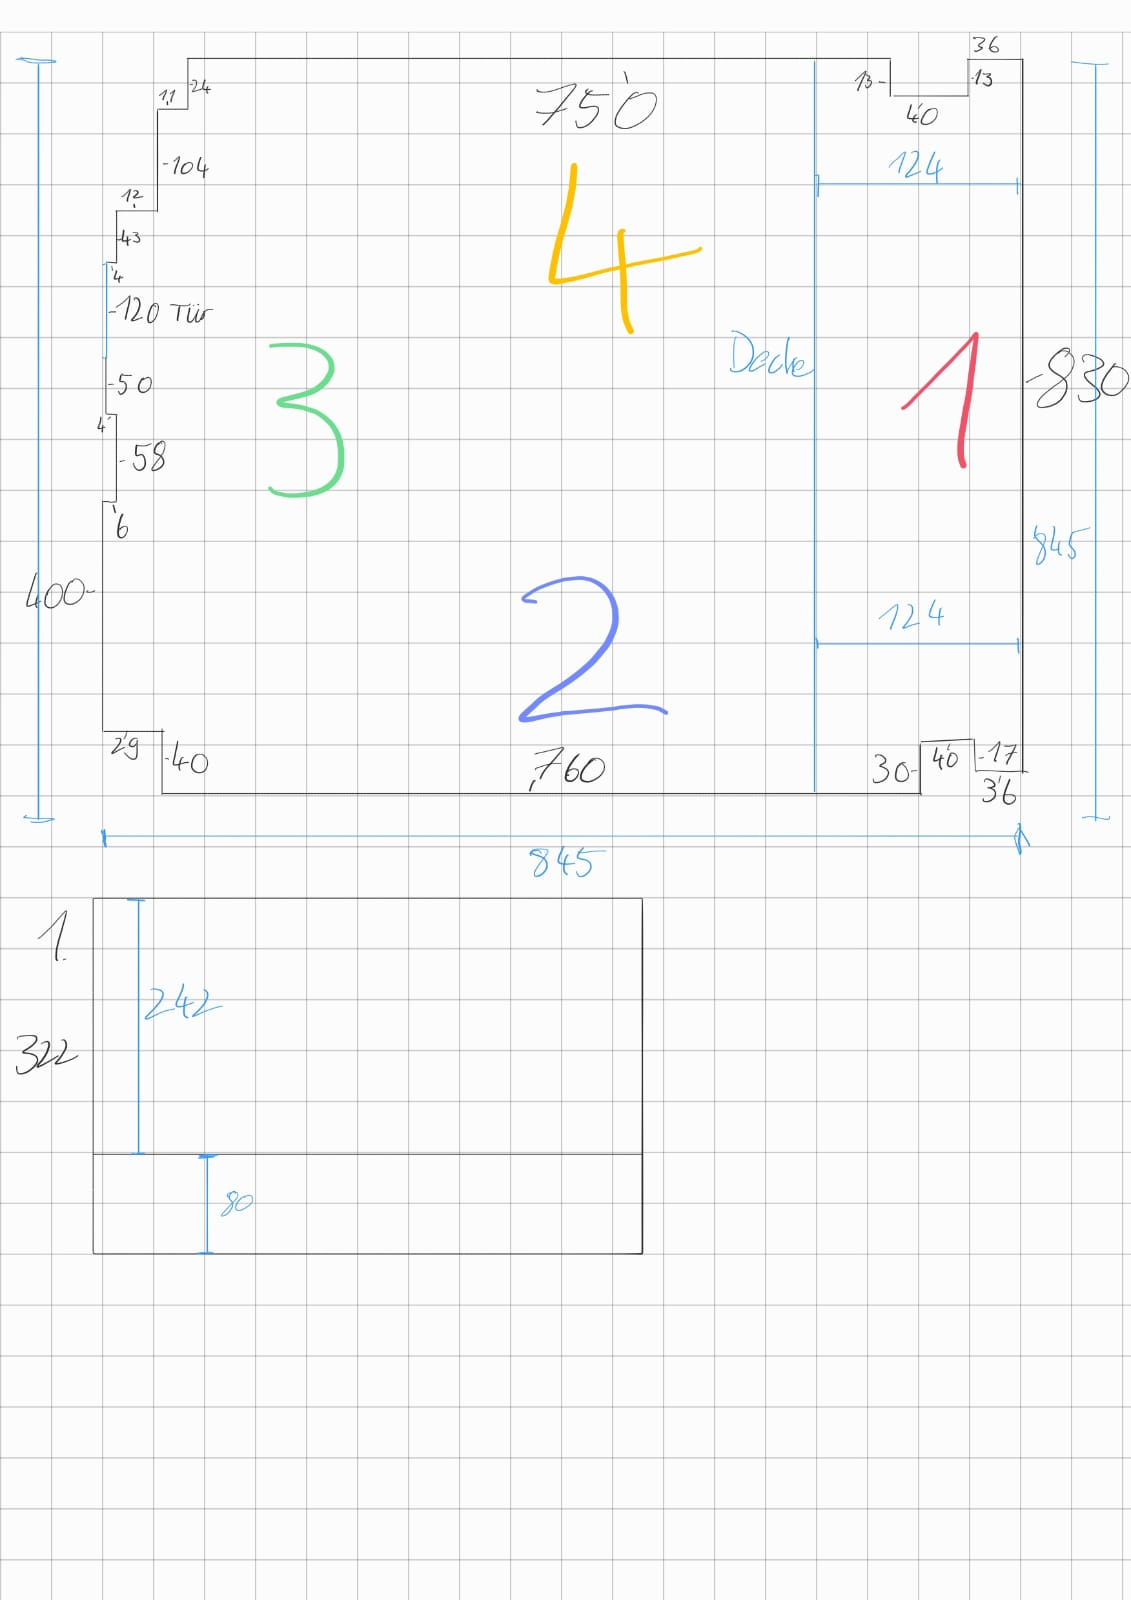
\includegraphics[width=1\textwidth]{../images/3D-Modell/technZeichnVL.jpeg}
\end{center}
Diese Zeichnung dient als Grundlage für die 3D-Modellierung des Raumes, welche in Blender durchgeführt wurde:
\begin{center}
  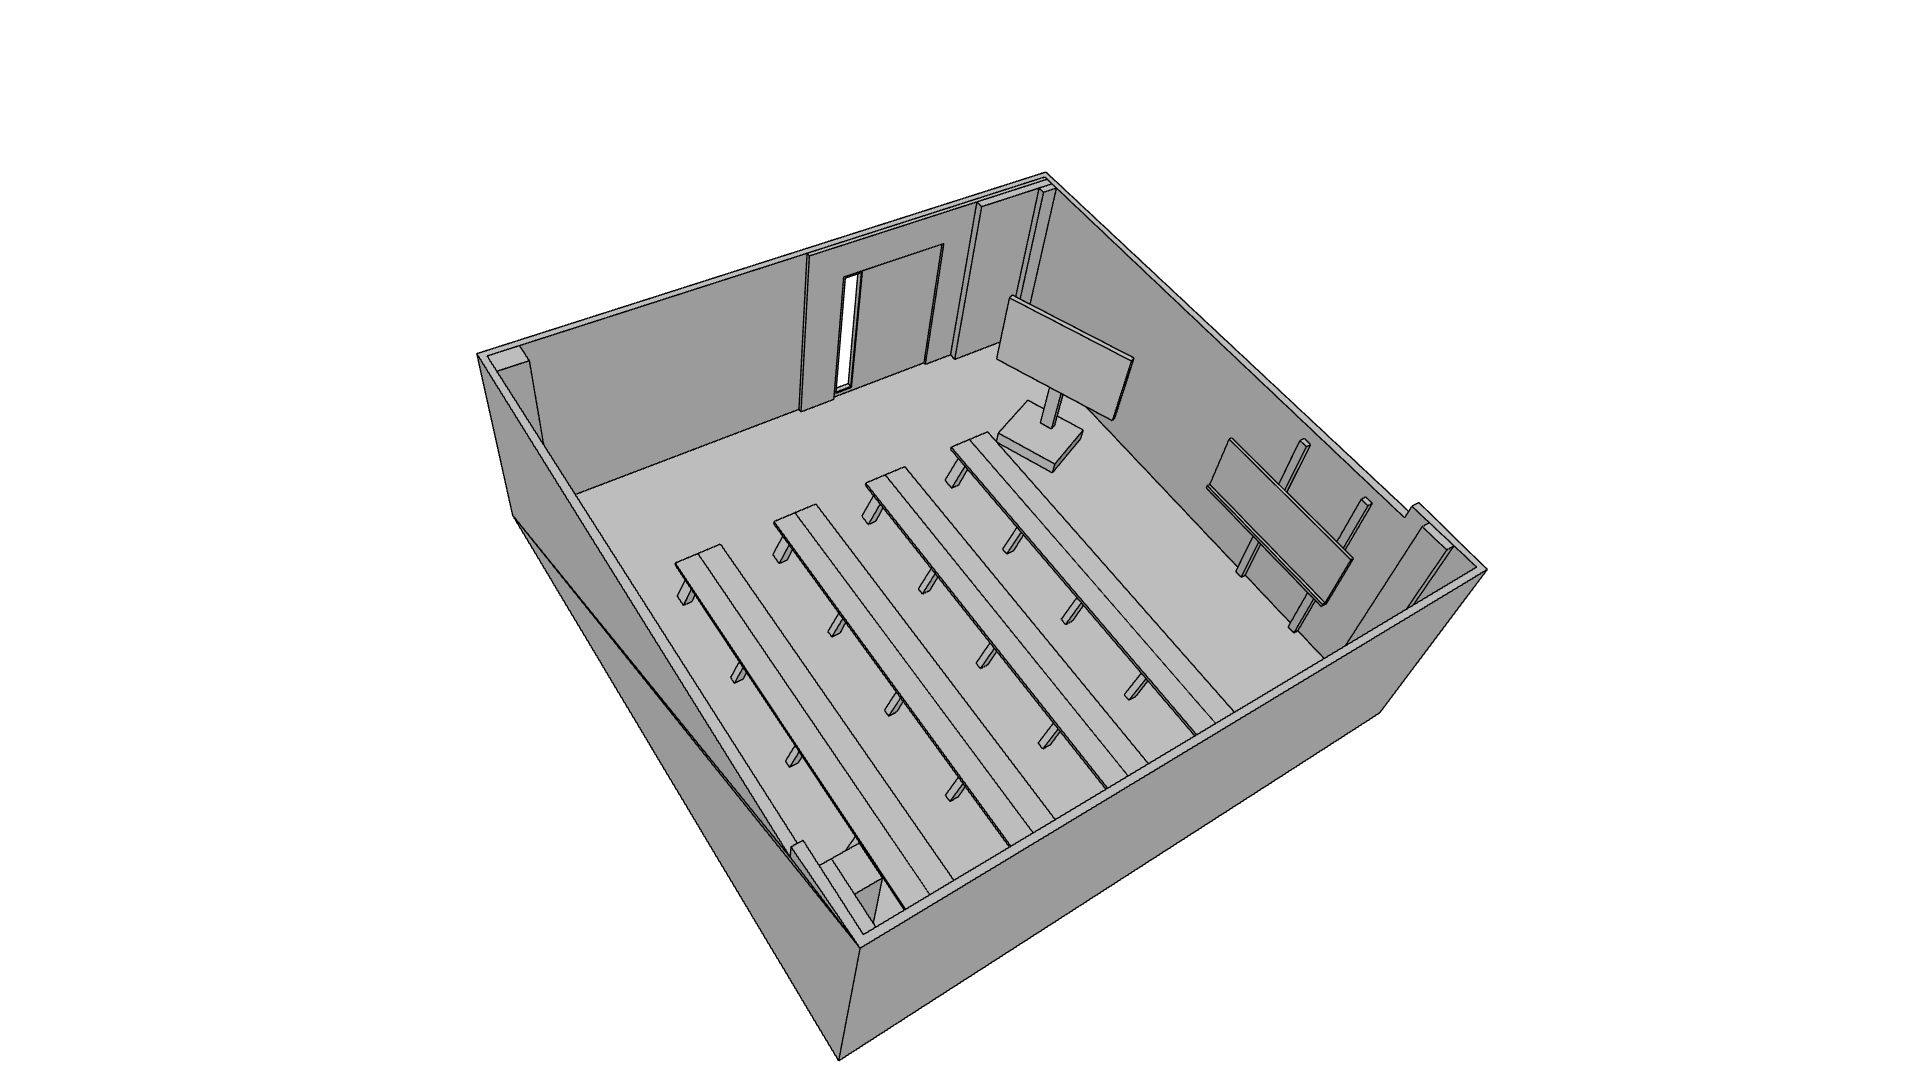
\includegraphics[width=1\textwidth]{../images/3D-Modell/VLModell.png}
\end{center}
	\chapter{Algorithmus zur Schallquellenlokalisierung}

In diesem Kapitel werden verschiedene Ansätze zur Lokalisierung einer Schallquelle im Raum beschrieben. Die Verfahren unterscheiden sich in ihrer physikalischen Genauigkeit, im Rechenaufwand sowie in der praktischen Umsetzbarkeit. Es werden sowohl rein mathematische Interpolationsverfahren als auch modellbasierte und lernbasierte Methoden betrachtet.

\section{Grundprinzipien}

Ein präziser, aber aktuell nicht umsetzbarer Ansatz wäre die \textit{Time Difference of Arrival} (TDOA) in Kombination mit Beamforming. Dabei wird die Zeitdifferenz der Schallausbreitung zwischen mehreren Mikrofonen gemessen. Über Verfahren wie Trilateration oder GCC-PHAT lassen sich daraus Einfallswinkel und Quelle berechnen.  
Da die vorhandene Hardware jedoch keine ausreichend genaue Zeitmessung erlaubt, konnte dieser Ansatz bislang nicht praktisch umgesetzt werden.

\section{Betrachtete Verfahren}

\textbf{Bilineare Interpolation:}  
Aus den vier Eckpunkten eines Messrasters wird durch zweifache lineare Interpolation eine flache Ebene gebildet. Dies liefert eine gleichmäßige, symmetrische Heatmap, berücksichtigt jedoch keinerlei physikalische Eigenschaften der Schallausbreitung. Damit eignet sich die Methode eher zur Visualisierung als zur tatsächlichen Lokalisierung.
\begin{lstlisting}[language=JavaScript, caption={Bilineare Interpolation}]
for (let row = 0; row < 10; row++) {
  const y = row / 9;
  const rowData = [];
  for (let col = 0; col < 10; col++) {
    const x = col / 9;
    const V =
      sensorValues.d1 * (1 - x) * (1 - y) +
      sensorValues.d2 * x * (1 - y) +
      sensorValues.d3 * (1 - x) * y +
      sensorValues.d4 * x * y;
    rowData.push(Number(V.toFixed(2)));
  }
  grid.push(rowData);
}
\end{lstlisting}
\begin{minipage}[b]{0.5\textwidth}
  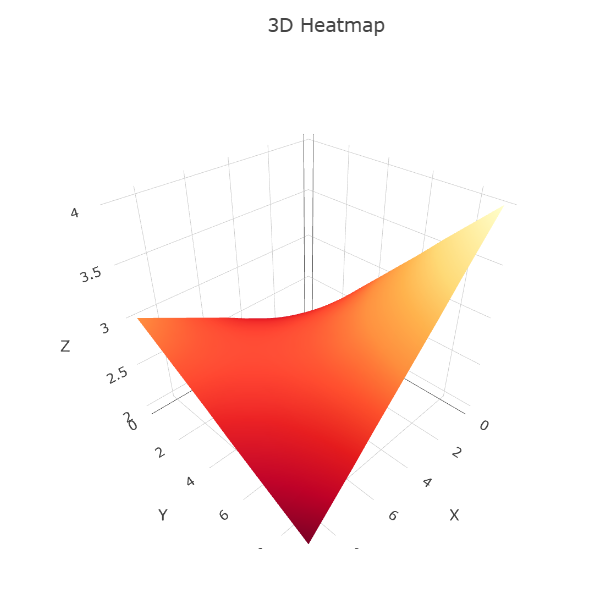
\includegraphics[width=\textwidth]{../images/Heatmap/IBHeatmap.png}
\end{minipage}

\textbf{Inverse Distance Weighting (IDW):}  
Hierbei wird der Einfluss eines Sensors umgekehrt proportional zur Distanz zur betrachteten Position gewichtet, häufig mit einem Distanzexponenten von $p=2$ (inverse quadratische Gewichtung). Das Ergebnis ist eine weiche Heatmap, deren Maximum meist in der Nähe der lautesten Sensoren liegt. Bei mehreren Schallquellen oder komplexer Raumakustik verschwimmt jedoch das Ergebnis.
\begin{lstlisting}[language=JavaScript, caption={Inverse Distance Weighting}]
const power = 2; // Distanzexponent
for (let row = 0; row < 10; row++) {
  const y = row / 9;
  const rowData = [];
  for (let col = 0; col < 10; col++) {
    const x = col / 9;
    let numerator = 0, denominator = 0;
    for (const [key, { x: sx, y: sy }] of Object.entries(sensorPositions)) {
      const value = sensorValues[key];
      const dx = x - sx;
      const dy = y - sy;
      const distance = Math.sqrt(dx * dx + dy * dy) || 0.0001;
      const weight = 1 / Math.pow(distance, power);
      numerator += value * weight;
      denominator += weight;
    }
    rowData.push(Number((numerator / denominator).toFixed(2)));
  }
  grid.push(rowData);
}
\end{lstlisting}
\begin{minipage}[b]{0.5\textwidth}
  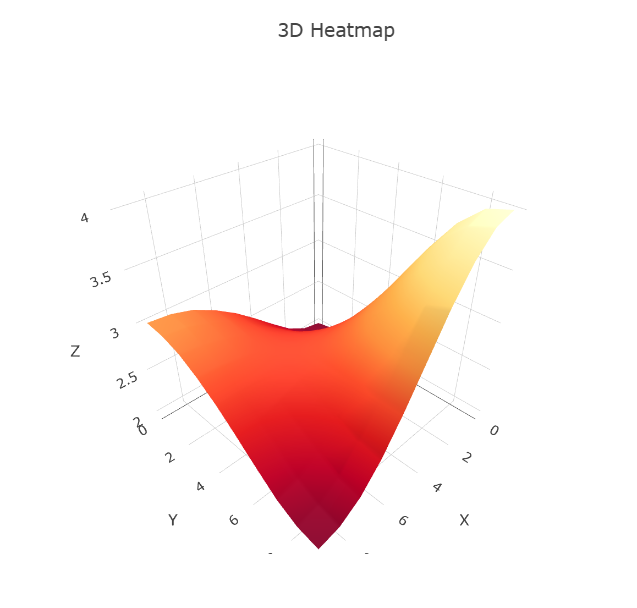
\includegraphics[width=\textwidth]{../images/Heatmap/IDWHeatmap.png}
\end{minipage}

\textbf{Physikalisches Modell – Rückwärtsprojektion:}  
Für jeden Punkt im Raum wird der erwartete Pegel an jedem Mikrofon berechnet:
\[
L = L_0 - 20 \cdot \log_{10}(d)
\]
mit $d$ als Abstand zwischen Quelle und Mikrofon. Anschließend werden die berechneten Werte mit den real gemessenen Pegeln verglichen und die Abweichungen gespeichert. Eine Heatmap zeigt die Positionen mit den geringsten Fehlern als wahrscheinlichste Quelle an.

\textbf{Maximum Likelihood Estimation (MLE):}  
Dieser statistische Ansatz modelliert die Wahrscheinlichkeit, dass eine Quelle an Position $(x, y)$ die gemessenen Pegel $s_i$ erzeugt:
\[
P = \prod_{i=1}^{n} \frac{1}{\sqrt{2\pi\sigma^2}} \cdot
\exp\left(-\frac{(s_i - (L_0 - 20\log_{10} d_i))^2}{2\sigma^2}\right)
\]
Der Punkt mit der höchsten Wahrscheinlichkeit wird als Quellenposition angenommen. Das Verfahren ist robust gegenüber Rauschen, erfordert jedoch ein präzises Modell für Messfehler.

\textbf{Weighted Centroid Localization (WCL):}  
Jeder Sensorwert wirkt wie eine „Gravitationskraft“, die die geschätzte Quelle in seine Richtung zieht. Durch Berechnung des gewichteten Mittelpunkts aller Sensoren lässt sich eine einzelne $(x,y)$-Position bestimmen, die den Schwerpunkt der Schallstärke darstellt. Gut geeignet, wenn ein dominanter Bereich im Raum deutlich lauter ist.
\begin{lstlisting}[language=JavaScript, caption={Weighted Centroid Localization (WCL)}]
	power = 2;    
  for (const [key, { x, y }] of Object.entries(sensorPositions)) {
    const value = sensorValues[key];
    const weight = Math.pow(value, power);
    weightedX += x * weight;
    weightedY += y * weight;
    weightSum += weight;
  }
\end{lstlisting}
\begin{minipage}[b]{0.5\textwidth}
  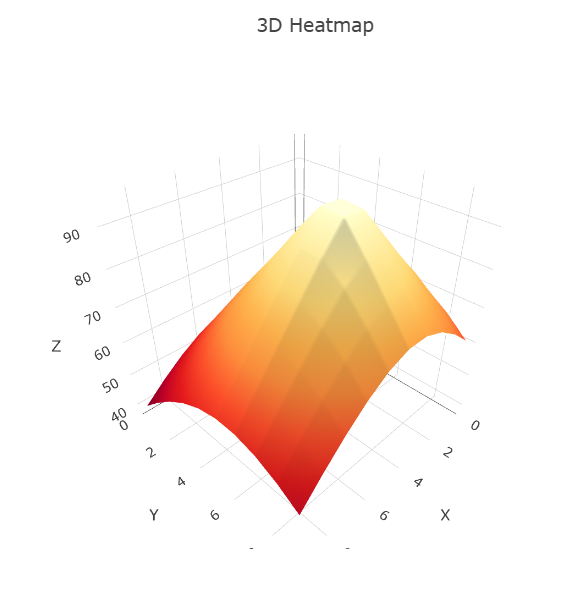
\includegraphics[width=\textwidth]{../images/Heatmap/WCLHeatmap.png}
\end{minipage}

\textbf{Machine Learning:}  
Durch Training eines Modells (z. B. KNN, Random Forest, MLP) mit bekannten Quellenpositionen und zugehörigen Pegelwerten kann die Quellenposition direkt aus den Messwerten vorhergesagt werden. Bei guter Trainingsbasis liefert dies sehr schnelle und präzise Ergebnisse. Allerdings sind umfangreiche und repräsentative Trainingsdaten erforderlich.

\textbf{Kombinierter IDW-WCL-Ansatz:}  
Zur Verbesserung der Lokalisierungsgenauigkeit wird zunächst eine IDW-Heatmap berechnet. Anschließend wird der durch WCL ermittelte Schwerpunkt durch einen zusätzlichen Peak (z. B. Gauß-Blob) verstärkt und in die Heatmap eingeblendet. Dadurch lassen sich weiche Verteilungen mit einem klaren Maximum kombinieren.
\begin{lstlisting}[language=JavaScript, caption={Kombinierter IDW-WCL-Ansatz}]
    for (let row = 0; row < gridSize; row++) {
      const y = row / (gridSize - 1);
      const rowData = [];

      for (let col = 0; col < gridSize; col++) {
        const x = col / (gridSize - 1);
        let numerator = 0;
        let denominator = 0;

        for (const point of interpolationPoints) {
          const dx = x - point.x;
          const dy = y - point.y;
          const distance = Math.sqrt(dx * dx + dy * dy) || epsilon;
          const weight = 1 / Math.pow(distance, idwFlatteningPower);
          numerator += point.value * weight;
          denominator += weight;
        }

        const interpolatedValue = numerator / denominator;
        rowData.push(Number(interpolatedValue.toFixed(2)));
      }

      grid.push(rowData);
    }
\end{lstlisting}
\begin{minipage}[b]{0.5\textwidth}
  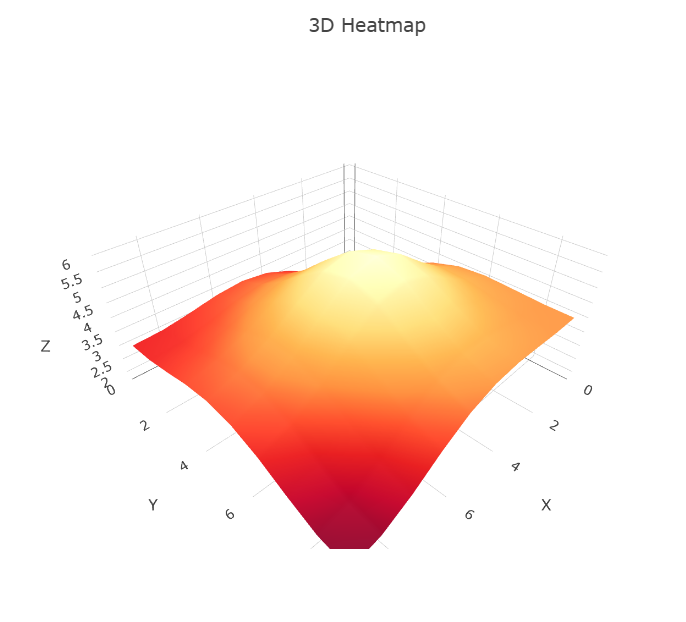
\includegraphics[width=\textwidth]{../images/Heatmap/IDWWCLHeatmap.png}
\end{minipage}

\section{Vergleich der Verfahren}

\begin{center}
\renewcommand{\arraystretch}{1.2}
\begin{adjustbox}{max width=\textwidth}
\begin{tabular}{|l|l|p{3cm}|p{3cm}|p{2.3cm}|}
\hline
\textbf{Methode} & \textbf{Typ} & \textbf{Vorteile} & \textbf{Nachteile} & \textbf{Quelle bestimmbar?} \\
\hline
Bilineare Interpolation & Interpolation & Schnell, symmetrische Heatmap & Kein physikalischer Bezug & Ungefähr \\
\hline
IDW & Interpolation & Einfach, intuitiv, glatte Heatmap & Kein klares Maximum & Ungefähr \\
\hline
Physikalisches Modell & Modellbasiert & Realitätsnah & Rechenintensiv, Annahmen nötig & Ja (Heatmap) \\
\hline
MLE & Wahrscheinlichkeit & Robust, statistisch fundiert & Modell für Fehler nötig & Ja (Wahrscheinlichkeit) \\
\hline
WCL & Schätzwert & Einfach, schneller Indikator & Ungenau bei asymmetrischen Verteilungen & Ja (Koordinate) \\
\hline
Machine Learning & Lernbasiert & Sehr schnell nach Training & Trainingsdaten nötig & Ja (xy direkt) \\
\hline
\end{tabular}
\end{adjustbox}
\end{center}

\section{Fazit}

Aus den Tests ergeben sich folgende Tendenzen:  
\begin{itemize}
    \item \textbf{Machine Learning} liefert bei guter Umsetzung die besten Ergebnisse, ist jedoch mit hohem Initialaufwand verbunden.
    \item \textbf{WCL} eignet sich gut, um den ungefähren Lautstärkenschwerpunkt im Raum zu bestimmen.
    \item \textbf{IDW} ist hilfreich, um Unterschiede in der Schallverteilung („hinten lauter als vorne“) darzustellen.
    \item \textbf{MLE} bietet hohes Potenzial für präzise Ortung, ist jedoch rechenintensiv und komplex in der Parametrisierung.
\end{itemize}

Eine Kombination aus IDW und WCL hat sich als vielversprechend erwiesen, um eine aussagekräftige Heatmap mit einem klar erkennbaren Maximum zu erzeugen.
Zudem ist diese Methode relativ einfach zu implementieren und benötigt keine aufwändige Kalibrierung.
Die Heatmap wird mit aktuellen Daten getestet, somit kann der Algorythmus durch die gewichtung von IDW und WCL angepasst werden.	
	\chapter{API-Kommunikation}
In diesem Kapitel wird die Kommunikation zwischen Frontend und Backend beschrieben, insbesondere die Übertragung von Heatmap-Daten. Es werden verschiedene Ansätze zur Datenübertragung und -kompression vorgestellt, um die Effizienz und Performance der Anwendung zu optimieren.
\section{Datenmengen und Optimierungsansätze}

\subsection{Problemstellung}
Wenn für jede Slider-Position eine API-Abfrage durchgeführt wird:
\begin{itemize}
    \item Bei einer Frequenz von 10~Hz (alle 100\,ms ein Datenpaket) ergeben sich 36{,}000 Zeitpunkte pro Sensor und somit 144{,}000 Werte pro Stunde.
    \item Beispielrechnung: $36{,}000 \times 10 \times 10 = 3{,}6$~Millionen Werte für ein $10\times10$-Array.
\end{itemize}

\subsection{Datenbasis}
\begin{itemize}
    \item \textbf{Heatmap-Größe:} $10\times10$ Werte (100 Felder pro Heatmap)
    \item \textbf{Datentyp:} Float16 (2~Byte pro Wert)
    \item \textbf{Frequenz:} 10~Hz (alle 100\,ms ein Frame)
    \item \textbf{Beispiel:} 1 Stunde = 3{,}600 Sekunden = 36{,}000 Frames
\end{itemize}

\noindent\textbf{Speicherbedarf (unkomprimiert):}
\[
100 \cdot 2\ \text{Bytes} = 200\ \text{Bytes/Frame}
\]
\[
200 \cdot 36{,}000 = 7{,}200{,}000\ \text{Bytes} \approx 7.2\ \text{MB}
\]

\subsection{Optimierungsoptionen}
\begin{enumerate}
    \item \textbf{Downsampling (Mittelwert pro Sekunde)} \\
    3{,}600 Frames/h → $3{,}600 \times 100$ Werte = 0.72\,MB.  
    Vorteil: geringe Datenmenge, einfaches JSON; Nachteil: Peaks nicht sichtbar.
    \item \textbf{Textkompression (Gzip/Brotli)} \\
    Reduktion auf ca. 15–25\,\% → $\approx 1.8$\,MB.
    \item \textbf{Binärformate (MessagePack, Protobuf, FlatBuffers)} \\
    30–40\,\% Ersparnis gegenüber JSON → $\approx 5.0$\,MB.
    \item \textbf{Binär + Kompression} \\
    Kombination aus beidem → $\approx 1.2$\,MB.
    \item \textbf{Delta-Encoding (nur Änderungen)} \\
    Angenommen: jeder 3.~Wert ändert sich → $\approx 3.4$\,MB.
    \item \textbf{Delta-Encoding + Kompression} \\
    Weitere Reduktion auf $\approx 1.0$–$1.2$\,MB.
    \item \textbf{Pre-Exportierte Dateien} \\
    Backend exportiert pro Stunde eine Datei → $\approx 7.2$\,MB.
    \item \textbf{Pre-Export + Kompression} \\
    Speicherbedarf: $\approx 1.2$\,MB/h; sehr performant und cachebar.
\end{enumerate}

\subsection{Vergleich der Ansätze}

\begin{center}
\begin{adjustbox}{max width=\textwidth}
\begin{tabular}{|l|c|p{5cm}|p{5cm}|}
\hline
\textbf{Beschreibung} & \textbf{Speicher/h} & \textbf{Vorteile} & \textbf{Nachteile} \\ \hline
Mittelwert pro Sekunde (Downsampling) & $\approx 0.72$\,MB & Sehr leicht, JSON möglich, wenig Traffic & Daten stark geglättet, Peaks nicht sichtbar \\ \hline
JSON + Gzip/Brotli & $\approx 1.8$\,MB & Einfach umsetzbar, keine großen Änderungen & Höhere Lesezeit, trotzdem noch Textformat \\ \hline
Binärformat & $\approx 5.0$\,MB & Schnell zu dekodieren, weniger Overhead & Komplexere Integration im Frontend \\ \hline
Binär + Kompression & $\approx 1.2$\,MB & Gute Mischung aus Effizienz \& Geschwindigkeit & Backend-Implementierung aufwändiger \\ \hline
Delta-Encoding & $\approx 3.5$\,MB & Ideal bei geringen Änderungen & Schlecht bei stark variablen Daten \\ \hline
Delta + Kompression & $1.0$–$1.2$\,MB & Sehr gute Kompression & Schwer zu debuggen, komplex \\ \hline
Pre-Export (roh) & $\approx 7.2$\,MB & Kein Runtime-Rechenaufwand, einfaches Caching & Hoher Speicherbedarf \\ \hline
Pre-Export + Kompression & $\approx 1.2$\,MB & Sehr performant, cachebar, ideal für Slider & Dateiverwaltung nötig \\ \hline
\end{tabular}
\end{adjustbox}
\end{center}

\subsection*{Fazit}
Aufgrund der hohen Komplexität und der großen Datenmengen ist es sinnvoll, die Heatmap-Arrays in einer separaten Datenbasis zu speichern. 
Das Frontend erhält die Daten in vorverarbeiteter Form durch Downsampling, um die Übertragungsmenge zu reduzieren und die Darstellungsgeschwindigkeit zu erhöhen. 
Zusätzlich wird eine Komprimierung der Daten in Betracht gezogen, um den Speicher- und Bandbreitenbedarf weiter zu minimieren, ohne die wesentliche Aussagekraft der Werte zu verlieren.

	\chapter{Benutzeroberfläche(UI)}
\section{Konzeption}
Während der Entwicklung wurde ein einfaches Frontend zu Testzwecken angelegt. 
Deshalb soll nun ein Plan entwickelt werden, wie die Benutzeroberfläche aussehen soll und welche Funktionen sie bieten soll:
\begin{center}
  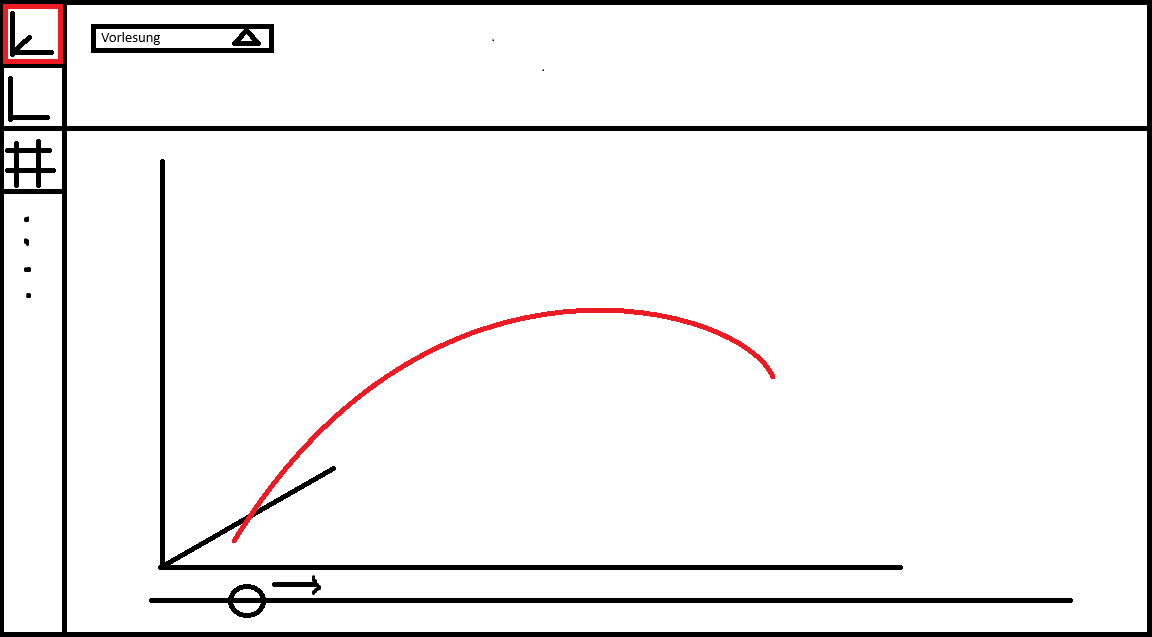
\includegraphics[width=1\textwidth]{../images/UI/SkizzeUI.png}
\end{center}
In dieser Skizze wurden die Grundfunktionen der Benutzeroberfläche festgelegt und die Anordnung der einzelnen Elemente skizziert.
Über eine Navbar an der linken Seite kann zwischen den einzelnen Seiten gewechselt werden. 
Auf der Hauptseite wird eine Heatmap angezeigt, die die Lautstärkeverteiung im Vorlesungsraum räumlich darstellt, wobei mit einem Dropdown-Menü der anzuzueigende Zeitraum ausgewählt werden kann.
Durch den ausgewählten Zeitraum kann anschließend mit einem Schieberegler die Zeit ausgewählt werden, für die die Lautstärke angezeigt werden soll.
Im nächsten Nav-Item sollen die einzelnen 2D-Grafen der jeweiligen Sensoren angezeigt werden. 
Das dritte Nav-Item soll einen tabellarischen Überblick über die gesammelten Daten geben, die in der Datenbank gespeichert sind.
Die Nvabar bietet Raum für zukünfitge Erweiterungen.
	% Anhang
	\clearpage
	\pagenumbering{roman}

	% Abbildungsverzeichnis
	%\cleardoublepage
	%\phantomsection \label{listoffig}
	%\addcontentsline{toc}{chapter}{Abbildungsverzeichnis}
	%\listoffigures

	%Tabellenverzeichnis
	%\cleardoublepage
	%\phantomsection \label{listoftab}
	%\addcontentsline{toc}{chapter}{Tabellenverzeichnis}
	%\listoftables

	% Quellcodeverzeichnis
	%\cleardoublepage
	%\phantomsection \label{listoflist}
	%\addcontentsline{toc}{chapter}{Listings}
	%\lstlistoflistings

	% Literaturverzeichnis
	\cleardoublepage
	\phantomsection \label{listoflit}
	\addcontentsline{toc}{chapter}{Literaturverzeichnis}
	
	%Bib style
	\bibliographystyle{agsm} %Havard
	%\bibliographystyle{amsplain} %Durchnummeriert
	%\bibliographystyle{amsalpha} %Kürzel für Autor und Jahr
	%see more: http://amath.colorado.edu/documentation/LaTeX/reference/faq/bibstyles.pdf
	
	\bibliography{ArbeitBib}

	% Abkürzungsverzeichnis
	%\cleardoublepage
	%\phantomsection \label{listofacs}
	%\addcontentsline{toc}{chapter}{Abkürzungsverzeichnis}
	%\input{ads/acronyms}
	
	% Glossar
	%\printglossary[style=altlist,title=Glossar]
\end{document}
